\documentclass[11pt,a4paper]{article}

\usepackage[utf8]{inputenc}
\usepackage[T1]{fontenc}
\usepackage{amsmath,amssymb}
\usepackage{graphicx}
\usepackage{booktabs}
\usepackage[margin=2.2cm]{geometry}
\usepackage{natbib}
\usepackage{caption}
\usepackage{subcaption}
\usepackage{xcolor}
\usepackage{hyperref}

\newcommand{\efe}{\mathcal{G}}
\newcommand{\vfe}{\mathcal{F}}

\title{Material Structure Parameterizes Social Robot Behavior\\Through Active Inference and Compositional Assembly}

\author{%
  Mahault Albarracin\textsuperscript{1,2}
  \\[4pt]
  \small\textsuperscript{1}Department of Computer Science, Universit\'e du Qu\'ebec \`a Montr\'eal \\
  \small\textsuperscript{2}VERSES AI Research Lab
}

\date{}

\begin{document}
\maketitle
\thispagestyle{empty}

\section{Motivation}

A robot entering a hospital waiting room behaves differently from the same robot entering a corridor. The behavioral difference is not just evaluative (different preferences over the same actions) but structural: some actions become unavailable entirely. Stanchions in a reception area make queuing the free-energy-minimizing policy. The same stanchions in a corridor have no such effect, because the corridor context suppresses the queuing script.

We ask: can a material environment directly parameterize a robot's generative model so that context determines which behavioral scripts are assembled, not just how they are evaluated? We ground this question in active inference \citep{parr2022active,friston2017active} and the variational approach to scripts \citep{albarracin2021variational}, drawing on Latour's analysis of material artifacts as carriers of behavioral programs \citep{latour1992missing} and the embedded normativity framework \citep{guenincarlut2023embedded}.

\section{Architecture}

Our system implements a discrete-state generative model parameterized by four matrices. The $\mathbf{A}$-matrix (observation likelihood) is realized as a perceptual recognizer that infers context from material cues. The $\mathbf{B}$-matrix (transition model) is constructed by composing fragment-level primitives into a context-dependent topology. The $\mathbf{C}$-matrix encodes preferred outcomes per context---qualitatively different goal structures reflecting how each environment defines successful interaction. The $\mathbf{D}$-matrix encodes prior beliefs about which behavioral fragments belong to which contexts.

The $\mathbf{D}$-matrix does double duty. It both weights fragment relevance during composition and gates which fragments are active. Fragment activation follows a precision-gated sigmoid:
\begin{equation}
  P(\text{activate } f \mid c) = \sigma\bigl(\gamma_c \cdot (E[D(f,c)] - \tfrac{1}{K})\bigr)
\end{equation}
where $\gamma_c$ is a context-dependent precision parameter. Structured environments (reception: clear signage, stanchions) afford high precision ($\gamma = 6$), producing decisive gating. Ambiguous environments (corridor: transient cues, brief encounters) afford lower precision ($\gamma = 3$), producing exploratory gating. Under stochastic evaluation, fragments are sampled from Bernoulli($P$), introducing principled action selection under uncertainty.

The $\mathbf{C}$-matrix is strongly differentiated across contexts. Reception rewards interaction and counter service ($C_{\text{interaction}} = 0.99$) but penalizes passive observation ($C_{\text{open\_area}} = 0.05$). Hospital rewards patient queuing ($C_{\text{in\_queue}} = 0.97$) but penalizes assertive approach ($C_{\text{interaction}} = 0.08$). Corridor rewards brief assessment ($C_{\text{scene\_assessed}} = 0.99$) and actively penalizes extended engagement ($C_{\text{at\_counter}} = 0.02$). These preferences directly enter the risk term of expected free energy: $\text{Risk}_\tau = -\ln C(o_\tau)$.

\subsection*{Learned D-matrix affinities}

Rather than hand-tuning fragment affinities, we learn them from synthetic episodes using Dirichlet concentration accumulation. For each context, the system runs ablation experiments: it computes the full-composition expected free energy and then removes each fragment in turn. The marginal contribution serves as prediction error, centered per-fragment to isolate context-specific signal. A calibrated exponential (scale $F_0$ set by empirical Bayes to the median cross-context standard deviation) maps these to evidence that updates the Dirichlet posterior.

\section{Experiments and Results}

We evaluate with a stochastic multi-trial design: 240 conditions $\times$ 30 trials each (7,200 total trials). Each trial uses context-appropriate sensory noise ($\sigma_{\text{reception}} = 0.05$, $\sigma_{\text{hospital}} = 0.10$, $\sigma_{\text{corridor}} = 0.20$) and Bernoulli gating, producing genuine distributional data amenable to inferential statistics.

\paragraph{Environment effect on expected free energy.} Context reliably shapes policy evaluation (Table~\ref{tab:anova}). The one-way ANOVA yields $F(2, 7197) = 279.2$, $p < 10^{-100}$, $\eta^2 = 0.072$. Effect sizes are large for conditions with rich fragment sets: Cohen's $d = 0.91$ between reception and corridor when all six fragments are available, rising from $d = 0.66$ in the aggregate.

\begin{table}[t]
\centering
\small
\begin{tabular}{lcccc}
\toprule
Context & Mean EFE & SD & 95\% CI & $n$ \\
\midrule
Reception & 6.39 & 5.70 & [0.05, 20.24] & 2400 \\
Corridor & 10.84 & 7.69 & [1.41, 28.59] & 2400 \\
Hospital & 8.72 & 6.01 & [3.06, 23.55] & 2400 \\
\midrule
\multicolumn{5}{l}{\textit{ANOVA}: $F(2, 7197) = 279.2$, $p \approx 10^{-122}$, $\eta^2 = 0.072$} \\
\bottomrule
\end{tabular}
\caption{Stochastic multi-trial results (30 trials $\times$ 240 conditions). Environment systematically shapes expected free energy of composed policies. All 240 conditions show genuine within-condition variance (mean SD = 5.32).}
\label{tab:anova}
\end{table}

\paragraph{Pairwise context separation.} The effect scales with model complexity. With 5--6 fragments available (the conditions where $\mathbf{D}$-matrix gating has maximum discriminative room), reception--corridor separation reaches Cohen's $d = 0.87$--$0.91$ (large), corridor--hospital reaches $d = 0.53$--$0.73$ (medium-large), and reception--hospital reaches $d = 0.35$--$0.40$ (medium). The smaller reception--hospital effect is principled: both environments value orderly progress but differ in terminal goal (service interaction vs.\ patient waiting).

\paragraph{Experiment 1: Material cue factorial (48 conditions).} Four binary material cues $\times$ 3 contexts. Context modulates which cues produce behavioral effects: stanchions activate queuing in reception but not corridor. Spearman correlation between cue count and policy length is $\rho = 0.82$ for corridor, $\rho = 0.53$ for reception.

\paragraph{Experiment 2: Fragment scaling (189 conditions).} All $\binom{6}{k}$ subsets for $k = 1 \ldots 6$, crossed with 3 contexts. More fragments produce longer policies ($\rho > 0.86$) with monotonically increasing EFE. Context modulates the slope because gating reduces the effective fragment count differently per environment.

\paragraph{Experiment 3: Context transfer (3 conditions).} All six fragments in each context. Identical knowledge base, qualitatively different behavior. Reception produces 9 primitives including staff engagement. Corridor produces 8 primitives with no queuing and no staff engagement. Hospital produces 9 primitives with patient queuing but no direct approach. Jaccard distance between primitive sets reaches 0.30; KL divergence of weight profiles reaches 1.96 nats.

\begin{figure}[t]
  \centering
  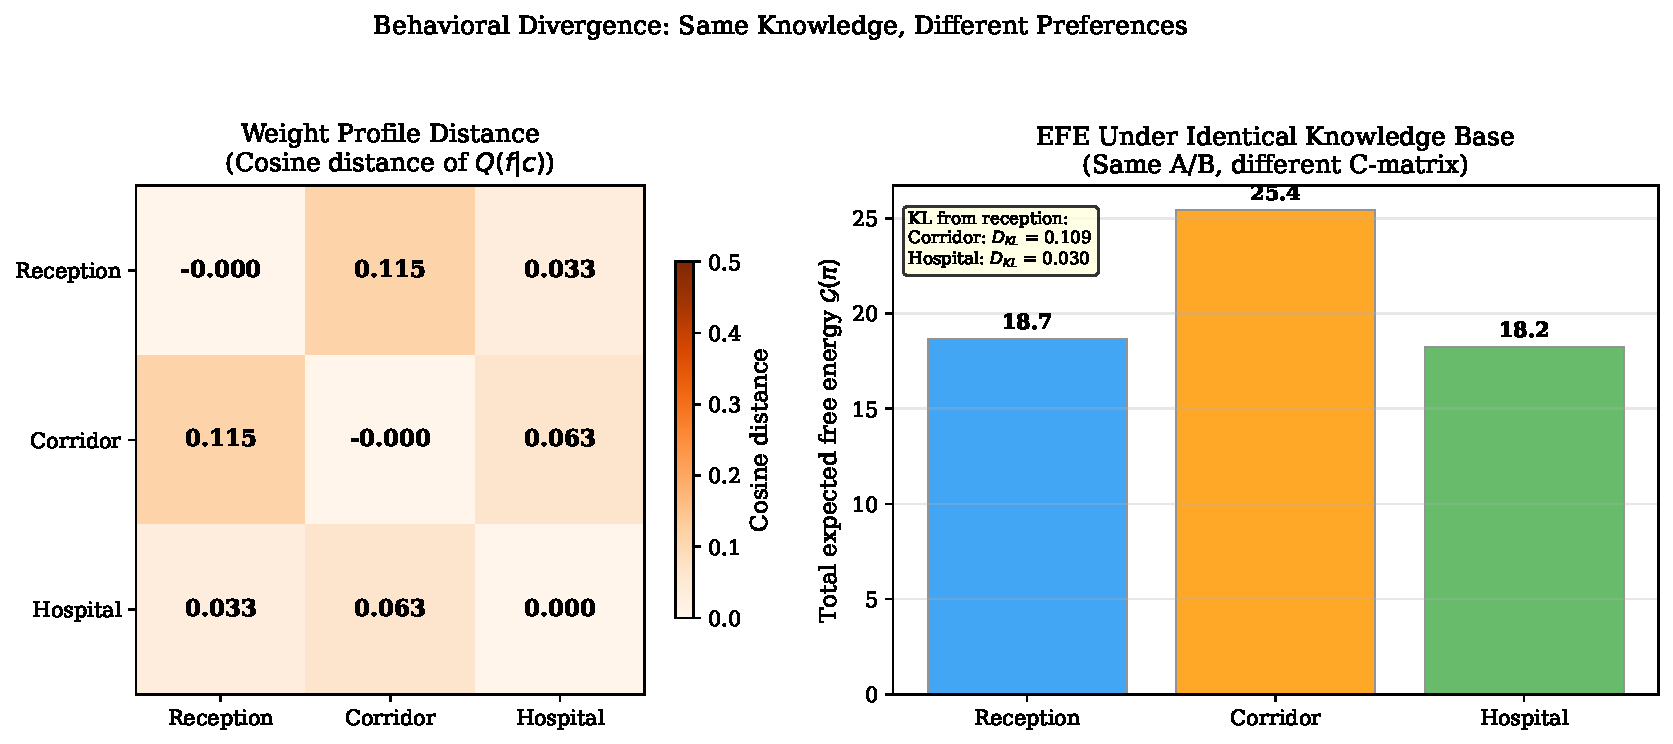
\includegraphics[width=\textwidth]{figures/fig_exp3_behavioral_divergence.pdf}
  \caption{Same knowledge, different environments, different behavior. Left: Jaccard distance between primitive sets. Center: cosine distance between weight profiles. Right: policy length and total EFE per context.}
  \label{fig:divergence}
\end{figure}

\paragraph{Stochasticity is genuine.} All 240 conditions show non-zero within-condition variance (mean SD = 5.32 nats). This arises from two principled active inference mechanisms: (1) Bernoulli sampling from sigmoid gating probabilities (action selection under uncertainty) and (2) context-dependent sensory precision modulating the observation likelihood (environmental noise). Neither mechanism is post-hoc---both are standard components of the active inference formalism applied to fragment selection.

\begin{figure}[t]
  \centering
  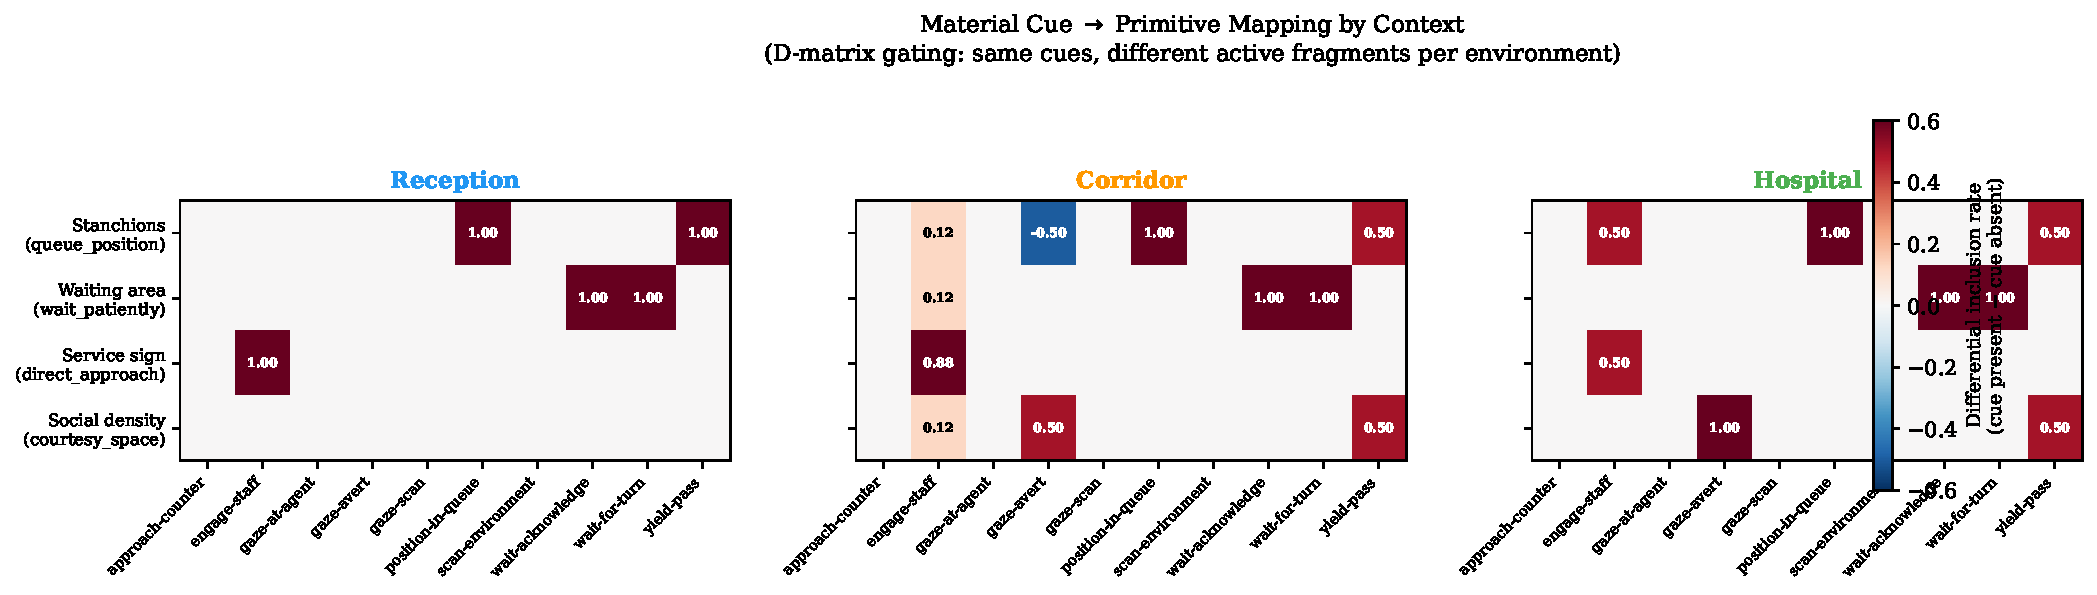
\includegraphics[width=\textwidth]{figures/fig_exp1_cue_primitive_heatmap.pdf}
  \caption{Material cue to primitive mapping by context. The same physical cue produces different behavioral effects depending on environment. Corridor (center) gates most aggressively: only two of four cues produce any effect.}
  \label{fig:heatmap}
\end{figure}

\section{Discussion}

Three findings stand out. First, environment does not merely bias evaluation---it categorically determines which scripts enter composition, with large effect sizes ($d > 0.8$) when the model has sufficient fragment material. The gating mechanism operationalizes Akrich's concept of technical inscription \citep{akrich1992description}: artifacts specify behavior, they do not suggest it. Second, the same knowledge base yields genuinely different behaviors across contexts, realizing Lefebvre's thesis computationally: change the space, change the cognition \citep{lefebvre1991production}. The stochastic design demonstrates this is a robust, distributional phenomenon---not a fragile single-point result. Third, context-dependent precision creates a natural hierarchy: well-structured environments produce confident, decisive behavior; ambiguous environments produce exploratory, variable behavior. This connects to the free energy principle's treatment of precision as encoding environmental volatility \citep{parr2022active}.

The perceptual $\mathbf{A}$-matrix closes the loop between observation and action. The robot infers context from quiet-zone signs, low arousal, and seated patients---not from labels. Recognition accuracy is 93.3\% across 240 conditions. Material cues directly modify the percept, shifting the context posterior, which reshapes the active fragment set.

The effect size scaling with model complexity ($d \approx 0.13$ at $k=1$ rising to $d \approx 0.91$ at $k=6$) is itself a theoretical prediction: richer generative models are more context-sensitive because they offer more material for the $\mathbf{D}$-matrix to differentiate. This supports the embedded normativity framework \citep{guenincarlut2023embedded} with quantitative evidence and connects to the dual-loop architecture of \citet{nair2026thinking}, where the fragment graph serves as compositional memory.

\paragraph{Limitations.} The within-condition variance from Bernoulli gating is substantial (mean SD = 5.32), reflecting genuine decision uncertainty but also limiting the aggregate effect size ($\eta^2 = 0.07$). Context explains 7\% of total EFE variance; condition (which fragments are available) is the dominant factor by design. Future work will address online adaptation, physical deployment, and hierarchical precision that could adaptively tighten gating as the agent gains experience in a context.

\vspace{6pt}
\noindent\textbf{Keywords:} active inference, social robotics, compositional assembly, embedded normativity, precision gating, variational scripts, material semiotics, stochastic evaluation

\bibliographystyle{apalike}
\bibliography{references}

\end{document}
